\documentclass[border=6pt]{standalone}
\usepackage{tikz}
\usetikzlibrary{arrows.meta,positioning,calc,shapes.geometric,fit,backgrounds,patterns,matrix,decorations.pathreplacing}
\begin{document}
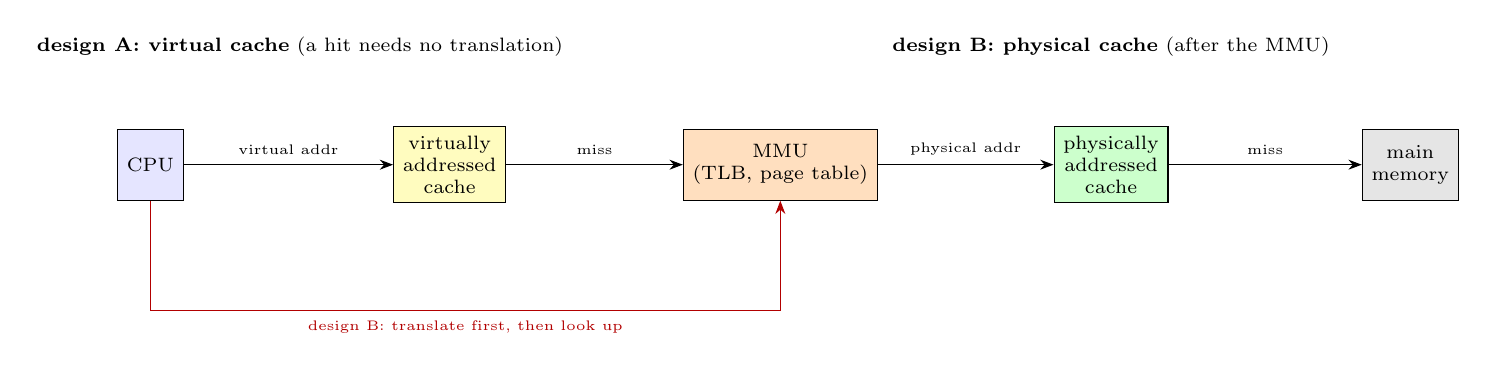
\begin{tikzpicture}[>=Stealth,font=\small]
\tikzstyle{b}=[draw,minimum height=0.9cm,align=center,font=\scriptsize]
\node[b,fill=blue!10] (cpu) at (0,0) {CPU};
\node[b,fill=yellow!25] (vc) at (3.8,0) {virtually\\ addressed\\ cache};
\node[b,fill=orange!25] (mmu) at (8,0) {MMU\\ (TLB, page table)};
\node[b,fill=green!20] (pc) at (12.2,0) {physically\\ addressed\\ cache};
\node[b,fill=gray!20] (mem) at (16,0) {main\\ memory};
\draw[->] (cpu) -- node[above,font=\tiny]{virtual addr} (vc);
\draw[->] (vc) -- node[above,font=\tiny]{miss} (mmu);
\draw[->] (mmu) -- node[above,font=\tiny]{physical addr} (pc);
\draw[->] (pc) -- node[above,font=\tiny]{miss} (mem);
\draw[->,red!70!black] (cpu.south) -- ++(0,-1.4) -| node[pos=0.25,below,font=\tiny,red!70!black]{design B: translate first, then look up} (mmu.south);
\node[font=\scriptsize,align=left] at (1.9,1.5) {\textbf{design A: virtual cache} (a hit needs no translation)};
\node[font=\scriptsize,align=left] at (12.2,1.5) {\textbf{design B: physical cache} (after the MMU)};
\end{tikzpicture}
\end{document}
